\documentclass{beamer}
\usepackage{tikz} % Figures
\usepackage{caption}
\usepackage{subcaption}
\usepackage{graphicx} % Images
\usepackage{color}

% To write formulas
\usepackage{amsfonts}
\usepackage{amsmath}

\usetheme{Darmstadt}

\newcommand\tab[1][1cm]{\hspace*{#1}}
 
\addtobeamertemplate{navigation symbols}{}{%
 \usebeamerfont{footline}%
 \usebeamercolor[fg]{footline}%
 \hspace{1em}%
 \insertframenumber/\inserttotalframenumber
}

\makeatletter
\setbeamertemplate{title page}{
	\begin{centering}
		\begin{beamercolorbox}[sep=8pt,center]{institute-graphics}
			\usebeamercolor[fg]{titlegraphic}\inserttitlegraphic
		\end{beamercolorbox}
		\begin{beamercolorbox}[sep=8pt,center]{title}
			\usebeamerfont{title}\inserttitle
		\end{beamercolorbox}
		\begin{beamercolorbox}[sep=8pt,center]{author-date}
			\usebeamerfont{author}\insertauthor \newline
			\usebeamerfont{date}\insertdate
		\end{beamercolorbox}
	\end{centering}
}
\makeatother
\title[Reducing Grenoble's car traffic]{\textsc{Decision Support System for carpooling to reduce car traffic in Grenoble area}}
\author{Romain NAVARRO}
\date{June, 29\textsuperscript{th} 2018}
\titlegraphic{\includegraphics[width=1.3cm]{img/l_uga}\hspace*{2.25cm}~%
	ORCO \hspace*{2.25cm}~%
	\includegraphics[width=1.3cm]{img/l_ensimag} \newline
	UGA \& ENSIMAG
}


\AtBeginSection[]{%
	\begin{frame}<beamer>
		\frametitle{Outline}
		\tableofcontents[sectionstyle=show/hide,subsectionstyle=show/show/hide]
	\end{frame}
	\addtocounter{framenumber}{-1}% Don't affect slide number
}

\begin{document}
	\begin{frame}[noframenumbering]
		\maketitle
		\begin{tabbing}
			Supervisor:\tab \= \textsc{Prof.} \=Van-Dat \textsc{CUNG}, G-SCOP \& UGA\\\medskip
			Jury members: \> \textsc{Prof.} \>Nadia \textsc{BRAUNER}\\
			\> \textsc{Prof.} \>Van-Dat \textsc{CUNG}\\
			\> \textsc{Dr.} \>Vassilissa \textsc{LEHOUX}\\
			\> \textsc{Prof.} \>Matej \textsc{STEHLIK}
		\end{tabbing}
	\end{frame}
	
	\begin{frame}
		\tableofcontents[hideallsubsections]
	\end{frame}
	%%%%%%%%%%%%% DEF OF THE GOAL %%%%%%%%%%
	\section{Context}
	\subsection{Carpooling}
	\begin{frame}[label=]
		\frametitle{Context: Carpooling}
		Carpooling characteristics:
		\begin{itemize}
			\item Private vehicles
			\item Group of people sharing the same car, called pool
			\item Participation in the expenses generated by the trips
		\end{itemize}
		\begin{figure}
			\includegraphics[width=5cm]{img/i_carpool}
		\end{figure}
	\end{frame}
	\subsection{Interests}
	\begin{frame}[label=]
		\frametitle{Context: Interests}
		Motivations:
		\begin{itemize}
			\item Users: Save money
			\item Communities: \begin{quote}With 20\% carpooling, there would be no traffic jams\end{quote} 
			\item Companies: Create a stronger sense of community and improve productivity
			\item Operators: Make money
		\end{itemize}
		\footnotetext[1]{Francois Bellot - fleeteurope.com}
		\footnotetext[2]{How to Encourage Employees to Carpool - rideamigos.com}
	\end{frame}
	\subsection{Existing applications}
	\begin{frame}[label=]
		\frametitle{Context: Existing applications}
		\begin{itemize}
			\item BlaBlaLines: Links users according to their schedule, allowing a detour of at most fifteen minutes for a trip
			\item Klaxit: Finds regular close carpoolers
			\item Karos: Fits with people who periodically do the same circuit
		\end{itemize}
		\footnotetext[1]{Covoiturage domicile-travail BlaBlaLines arrive Paris et en Ile-de-France - 2017}
		\footnotetext[2]{Sylvain Arnulf - Covoiturage domicile/travail : Klaxit (ex-Wayzup) embarque de nouveaux partenaires pour se detacher - 2018.}
		\footnotetext[3]{Karos, comment a marche ? - Le Parisien - 2016}
	\end{frame}
	\subsection{Barriers to these systems}
	\begin{frame}[label=]
		\frametitle{Context: Barriers to these systems}
		Three main barriers that emerge in the articles:
		\begin{itemize}
			\item Commitments: Users do not want to make a long-term commitment
			\item Punctuality: Users do not want to be too early or too late at work
			\item Detours: Users do not want to make too long detours
		\end{itemize}
		\footnotetext[1]{Hai-Jun Huang, Hai Yang, and Michael G. H. Bell. - 2000}
	\end{frame}
	
	%%%%%%%%% PRESENTATION OF THE PROBLEM %%%%%%%%%%
	\section{Problem description}
	\subsection{Same workplace for all}
	\begin{frame}
		\frametitle{Problem description: Same workplace for all}
		\begin{figure}
		\centering
		\begin{subfigure}{.5\textwidth}
			\centering
			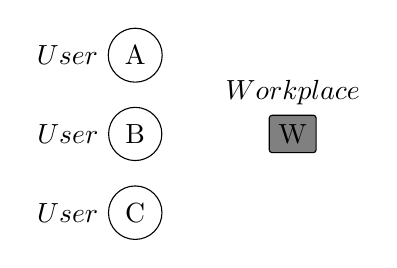
\begin{tikzpicture}
				\node[draw, circle, label=left:{$User$}] (A)at(-1.5, 0.5) {A};
				\node[draw, circle, label=left:{$User$}] (B)at(-1.5, -0.5) {B};
				\node[draw, circle, label=left:{$User$}] (C)at(-1.5, -1.5) {C};
				\node[draw, rectangle, rounded corners=1pt, fill=gray!100, label=above:{$Workplace$}] (W)at(0.5, -0.5) {W};
			\end{tikzpicture}
			\caption{User requests}
		\end{subfigure}%
		\begin{subfigure}{.5\textwidth}
			\centering
			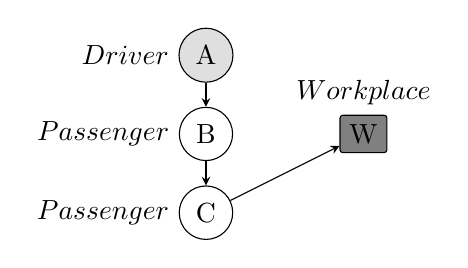
\begin{tikzpicture}
				\node[draw, circle, fill=gray!25, label=left:{$Driver$}] (A)at(-1.5, 0.5) {A};
				\node[draw, circle, label=left:{$Passenger$}] (B)at(-1.5, -0.5) {B};
				\node[draw, circle, label=left:{$Passenger$}] (C)at(-1.5, -1.5) {C};
				\node[draw, rectangle, rounded corners=1pt, fill=gray!100, label=above:{$Workplace$}] (W)at(0.5, -0.5) {W};
				\draw[->, >=stealth] (A) -- (B);
				\draw[->, >=stealth] (B) -- (C);
				\draw[->, >=stealth] (C) -- (W);
			\end{tikzpicture}
			\caption{A solution}
		\end{subfigure}
		\end{figure}
		\footnotetext[1]{Yuhan Guo - 2012}
	\end{frame}
	\subsection{One workplace per user}
	\begin{frame}
		\frametitle{Problem description: One workplace per user}
		\begin{figure}
		\centering
		\begin{subfigure}{.5\textwidth}
			\centering
			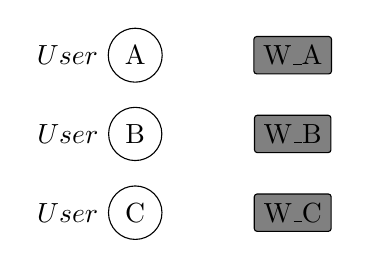
\begin{tikzpicture}
				\node[draw, circle, label=left:{$User$}] (A)at(-1.5, 0.5) {A};
				\node[draw, circle, label=left:{$User$}] (B)at(-1.5, -0.5) {B};
				\node[draw, circle, label=left:{$User$}] (C)at(-1.5, -1.5) {C};
				\node[draw, rectangle, rounded corners=1pt, fill=gray!100, label=right:{$$}] (WA)at(0.5, 0.5) {W\_A};
				\node[draw, rectangle, rounded corners=1pt, fill=gray!100, label=right:{$$}] (WB)at(0.5, -0.5) {W\_B};
				\node[draw, rectangle, rounded corners=1pt, fill=gray!100, label=right:{$$}] (WC)at(0.5, -1.5) {W\_C};
			\end{tikzpicture}
			\caption{User requests}
		\end{subfigure}%
		\begin{subfigure}{.5\textwidth}
			\centering
			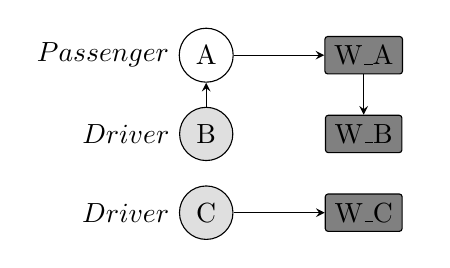
\begin{tikzpicture}
				\node[draw, circle, label=left:{$Passenger$}] (A)at(-1.5, 0.5) {A};
				\node[draw, circle, fill=gray!25, label=left:{$Driver$}] (B)at(-1.5, -0.5) {B};
				\node[draw, circle, fill=gray!25, label=left:{$Driver$}] (C)at(-1.5, -1.5) {C};
				\node[draw, rectangle, rounded corners=1pt, fill=gray!100, label=right:{$$}] (WA)at(0.5, 0.5) {W\_A};
				\node[draw, rectangle, rounded corners=1pt, fill=gray!100, label=right:{$$}] (WB)at(0.5, -0.5) {W\_B};
				\node[draw, rectangle, rounded corners=1pt, fill=gray!100, label=right:{$$}] (WC)at(0.5, -1.5) {W\_C};
				\draw[->, >=stealth] (C) -- (WC);
				\draw[->, >=stealth] (A) -- (WA);
				\draw[->, >=stealth] (WA) -- (WB);
				\draw[->, >=stealth] (B) -- (A);
			\end{tikzpicture}
			\caption{A solution}
		\end{subfigure}
		\end{figure}
		\footnotetext[1]{Yuhan Guo - 2012}
	\end{frame}
	\subsection{Work arrival time}
	\begin{frame}
		\frametitle{Problem description: Work arrival time}
		\begin{figure}
		\centering
		\begin{subfigure}{.5\textwidth}
			\centering
			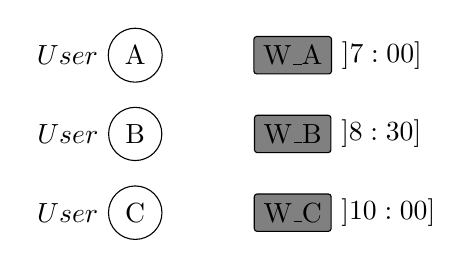
\begin{tikzpicture}
				\node[draw, circle, label=left:{$User$}] (A)at(-1.5, 0.5) {A};
				\node[draw, circle, label=left:{$User$}] (B)at(-1.5, -0.5) {B};
				\node[draw, circle, label=left:{$User$}] (C)at(-1.5, -1.5) {C};
				\node[draw, rectangle, rounded corners=1pt, fill=gray!100, label=right:{$]7:00]$}] (WA)at(0.5, 0.5) {W\_A};
				\node[draw, rectangle, rounded corners=1pt, fill=gray!100, label=right:{$]8:30]$}] (WB)at(0.5, -0.5) {W\_B};
				\node[draw, rectangle, rounded corners=1pt, fill=gray!100, label=right:{$]10:00]$}] (WC)at(0.5, -1.5) {W\_C};
			\end{tikzpicture}
			\caption{User requests}
		\end{subfigure}%
		\begin{subfigure}{.5\textwidth}
			\centering
			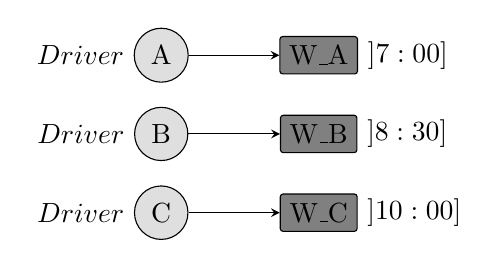
\begin{tikzpicture}
				\node[draw, circle, fill=gray!25, label=left:{$Driver$}] (A)at(-1.5, 0.5) {A};
				\node[draw, circle, fill=gray!25, label=left:{$Driver$}] (B)at(-1.5, -0.5) {B};
				\node[draw, circle, fill=gray!25, label=left:{$Driver$}] (C)at(-1.5, -1.5) {C};
				\node[draw, rectangle, rounded corners=1pt, fill=gray!100, label=right:{$]7:00]$}] (WA)at(0.5, 0.5) {W\_A};
				\node[draw, rectangle, rounded corners=1pt, fill=gray!100, label=right:{$]8:30]$}] (WB)at(0.5, -0.5) {W\_B};
				\node[draw, rectangle, rounded corners=1pt, fill=gray!100, label=right:{$]10:00]$}] (WC)at(0.5, -1.5) {W\_C};
				\draw[->, >=stealth] (C) -- (WC);
				\draw[->, >=stealth] (A) -- (WA);
				\draw[->, >=stealth] (B) -- (WB);
			\end{tikzpicture}
			\caption{A solution}
		\end{subfigure}
		\end{figure}
		\footnotetext[1]{Shangyao Yan and Chun-Ying Chen - 2011}
	\end{frame}
	
	\subsection{Objective}
	\begin{frame}
		\frametitle{Problem description: Objective}
		\begin{figure}
		\centering
		\begin{subfigure}{.5\textwidth}
			\centering
			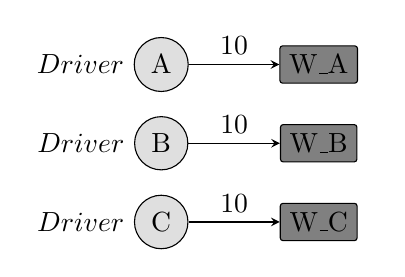
\begin{tikzpicture}
				\node[draw, circle, fill=gray!25, label=left:{$Driver$}] (A)at(-1.5, 0.5) {A};
				\node[draw, circle, fill=gray!25, label=left:{$Driver$}] (B)at(-1.5, -0.5) {B};
				\node[draw, circle, fill=gray!25, label=left:{$Driver$}] (C)at(-1.5, -1.5) {C};
				\node[draw, rectangle, rounded corners=1pt, fill=gray!100, label=right:{$$}] (WA)at(0.5, 0.5) {W\_A};
				\node[draw, rectangle, rounded corners=1pt, fill=gray!100, label=right:{$$}] (WB)at(0.5, -0.5) {W\_B};
				\node[draw, rectangle, rounded corners=1pt, fill=gray!100, label=right:{$$}] (WC)at(0.5, -1.5) {W\_C};
				\draw[->, >=stealth, above] (A) -- (WA) node[midway] {$10$};
				\draw[->, >=stealth, above] (B) -- (WB) node[midway] {$10$};
				\draw[->, >=stealth, above] (C) -- (WC) node[midway] {$10$};
			\end{tikzpicture}
			\caption{Total cost = 30}
		\end{subfigure}%
		\begin{subfigure}{.5\textwidth}
			\centering
			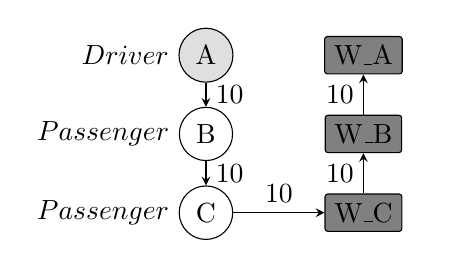
\begin{tikzpicture}
				\node[draw, circle, fill=gray!25, label=left:{$Driver$}] (A)at(-1.5, 0.5) {A};
				\node[draw, circle, label=left:{$Passenger$}] (B)at(-1.5, -0.5) {B};
				\node[draw, circle, label=left:{$Passenger$}] (C)at(-1.5, -1.5) {C};
				\node[draw, rectangle, rounded corners=1pt, fill=gray!100, label=right:{$$}] (WA)at(0.5, 0.5) {W\_A};
				\node[draw, rectangle, rounded corners=1pt, fill=gray!100, label=right:{$$}] (WB)at(0.5, -0.5) {W\_B};
				\node[draw, rectangle, rounded corners=1pt, fill=gray!100, label=right:{$$}] (WC)at(0.5, -1.5) {W\_C};
				\draw[->, >=stealth, right] (A) -- (B) node[midway] {$10$};
				\draw[->, >=stealth, right] (B) -- (C) node[midway] {$10$};
				\draw[->, >=stealth, left] (WC) -- (WB) node[midway] {$10$};
				\draw[->, >=stealth, above] (C) -- (WC) node[midway] {$10$};
				\draw[->, >=stealth, left] (WB) -- (WA) node[midway] {$10$};
			\end{tikzpicture}
			\caption{Total cost = 50}
		\end{subfigure}
		\caption{Minimization of the total cost}
		\end{figure}
		\footnotetext[1]{Jakub Nalepa - 2016}
	\end{frame}
	\subsection{Return management}
	\begin{frame}
		\frametitle{Problem description: Same pool}
		\begin{figure}
		\centering
		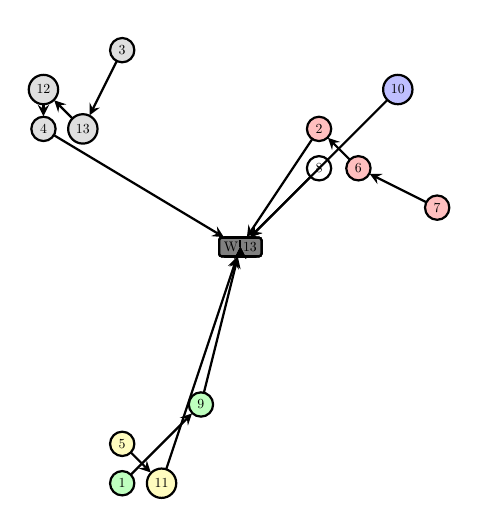
\begin{tikzpicture}[thick,scale=0.5, every node/.style={transform shape}]
			\node[draw,circle,fill=green!25,label=above:{$$}] (1)at(-3.0,-6.0) {1};
			\node[draw,circle,fill=red!25,label=above:{$$}] (2)at(2.0,3.0) {2};
			\node[draw,circle,fill=gray!25,label=above:{$$}] (3)at(-3.0,5.0) {3};
			\node[draw,circle,fill=gray!25,label=above:{$$}] (4)at(-5.0,3.0) {4};
			\node[draw,circle,fill=yellow!25,label=above:{$$}] (5)at(-3.0,-5.0) {5};
			\node[draw,circle,fill=red!25,label=above:{$$}] (6)at(3.0,2.0) {6};
			\node[draw,circle,fill=red!25,label=above:{$$}] (7)at(5.0,1.0) {7};
			\node[draw,circle,label=above:{$$}] (8)at(2.0,2.0) {8};
			\node[draw,circle,fill=green!25,label=above:{$$}] (9)at(-1.0,-4.0) {9};
			\node[draw,circle,fill=blue!25,label=above:{$$}] (10)at(4.0,4.0) {10};
			\node[draw,circle,fill=yellow!25,label=above:{$$}] (11)at(-2.0,-6.0) {11};
			\node[draw,circle,fill=gray!25,label=above:{$$}] (12)at(-5.0,4.0) {12};
			\node[draw,circle,fill=gray!25,label=above:{$$}] (13)at(-4.0,3.0) {13};
			\node[draw,rectangle,rounded corners=1pt,fill=gray!100,label=above:{$$}] (W1)at(0.0,0.0) {W\_1};
			\node[draw,rectangle,rounded corners=1pt,fill=gray!100,label=above:{$$}] (W2)at(0.0,0.0) {W\_2};
			\node[draw,rectangle,rounded corners=1pt,fill=gray!100,label=above:{$$}] (W3)at(0.0,0.0) {W\_3};
			\node[draw,rectangle,rounded corners=1pt,fill=gray!100,label=above:{$$}] (W4)at(0.0,0.0) {W\_4};
			\node[draw,rectangle,rounded corners=1pt,fill=gray!100,label=above:{$$}] (W5)at(0.0,0.0) {W\_5};
			\node[draw,rectangle,rounded corners=1pt,fill=gray!100,label=above:{$$}] (W6)at(0.0,0.0) {W\_6};
			\node[draw,rectangle,rounded corners=1pt,fill=gray!100,label=above:{$$}] (W7)at(0.0,0.0) {W\_7};
			\node[draw,rectangle,rounded corners=1pt,fill=gray!100,label=above:{$$}] (W8)at(0.0,0.0) {W\_8};
			\node[draw,rectangle,rounded corners=1pt,fill=gray!100,label=above:{$$}] (W9)at(0.0,0.0) {W\_9};
			\node[draw,rectangle,rounded corners=1pt,fill=gray!100,label=above:{$$}] (W10)at(0.0,0.0) {W\_10};
			\node[draw,rectangle,rounded corners=1pt,fill=gray!100,label=above:{$$}] (W11)at(0.0,0.0) {W\_11};
			\node[draw,rectangle,rounded corners=1pt,fill=gray!100,label=above:{$$}] (W12)at(0.0,0.0) {W\_12};
			\node[draw,rectangle,rounded corners=1pt,fill=gray!100,label=above:{$$}] (W13)at(0.0,0.0) {W\_13};
			\draw[->,>=stealth] (1) -- (9);
			\draw[->,>=stealth] (9) -- (W9);
			\draw[->,>=stealth] (W9) -- (W1);
			\draw[->,>=stealth] (3) -- (13);
			\draw[->,>=stealth] (4) -- (W13);
			\draw[->,>=stealth] (12) -- (4);
			\draw[->,>=stealth] (13) -- (12);
			\draw[->,>=stealth] (W4) -- (W3);
			\draw[->,>=stealth] (W12) -- (W4);
			\draw[->,>=stealth] (W13) -- (W12);
			\draw[->,>=stealth] (5) -- (11);
			\draw[->,>=stealth] (11) -- (W11);
			\draw[->,>=stealth] (W11) -- (W5);
			\draw[->,>=stealth] (2) -- (W6);
			\draw[->,>=stealth] (6) -- (2);
			\draw[->,>=stealth] (7) -- (6);
			\draw[->,>=stealth] (W2) -- (W7);
			\draw[->,>=stealth] (W6) -- (W2);
			\draw[->,>=stealth] (8) -- (W8);
			\draw[->,>=stealth] (10) -- (W10);
		\end{tikzpicture}
		\caption{Home-to-work user pools }
	\end{figure}
	\end{frame}
	\begin{frame}
		\frametitle{Problem description: Same pool}
\begin{figure}
		\centering
		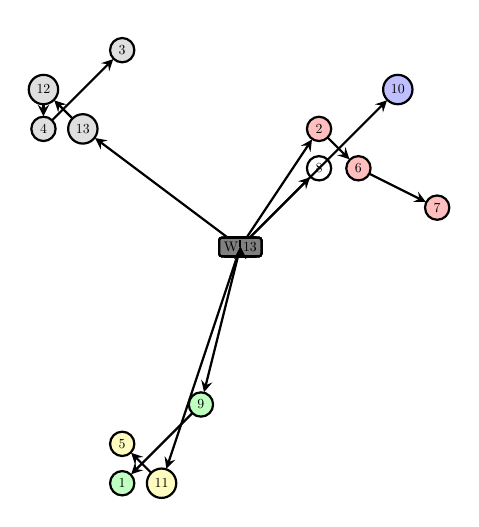
\begin{tikzpicture}[thick,scale=0.5, every node/.style={transform shape}]
			\node[draw,rectangle,rounded corners=1pt,fill=gray!100,label=above:{$$}] (W1)at(0.0,0.0) {W\_1};
			\node[draw,rectangle,rounded corners=1pt,fill=gray!100,label=above:{$$}] (W2)at(0.0,0.0) {W\_2};
			\node[draw,rectangle,rounded corners=1pt,fill=gray!100,label=above:{$$}] (W3)at(0.0,0.0) {W\_3};
			\node[draw,rectangle,rounded corners=1pt,fill=gray!100,label=above:{$$}] (W4)at(0.0,0.0) {W\_4};
			\node[draw,rectangle,rounded corners=1pt,fill=gray!100,label=above:{$$}] (W5)at(0.0,0.0) {W\_5};
			\node[draw,rectangle,rounded corners=1pt,fill=gray!100,label=above:{$$}] (W6)at(0.0,0.0) {W\_6};
			\node[draw,rectangle,rounded corners=1pt,fill=gray!100,label=above:{$$}] (W7)at(0.0,0.0) {W\_7};
			\node[draw,rectangle,rounded corners=1pt,fill=gray!100,label=above:{$$}] (W8)at(0.0,0.0) {W\_8};
			\node[draw,rectangle,rounded corners=1pt,fill=gray!100,label=above:{$$}] (W9)at(0.0,0.0) {W\_9};
			\node[draw,rectangle,rounded corners=1pt,fill=gray!100,label=above:{$$}] (W10)at(0.0,0.0) {W\_10};
			\node[draw,rectangle,rounded corners=1pt,fill=gray!100,label=above:{$$}] (W11)at(0.0,0.0) {W\_11};
			\node[draw,rectangle,rounded corners=1pt,fill=gray!100,label=above:{$$}] (W12)at(0.0,0.0) {W\_12};
			\node[draw,rectangle,rounded corners=1pt,fill=gray!100,label=above:{$$}] (W13)at(0.0,0.0) {W\_13};
			\node[draw,circle,fill=green!25,label=above:{$$}] (1)at(-3.0,-6.0) {1};
			\node[draw,circle,fill=red!25,label=above:{$$}] (2)at(2.0,3.0) {2};
			\node[draw,circle,fill=gray!25,label=above:{$$}] (3)at(-3.0,5.0) {3};
			\node[draw,circle,fill=gray!25,label=above:{$$}] (4)at(-5.0,3.0) {4};
			\node[draw,circle,fill=yellow!25,label=above:{$$}] (5)at(-3.0,-5.0) {5};
			\node[draw,circle,fill=red!25,label=above:{$$}] (6)at(3.0,2.0) {6};
			\node[draw,circle,fill=red!25,label=above:{$$}] (7)at(5.0,1.0) {7};
			\node[draw,circle,label=above:{$$}] (8)at(2.0,2.0) {8};
			\node[draw,circle,fill=green!25,label=above:{$$}] (9)at(-1.0,-4.0) {9};
			\node[draw,circle,fill=blue!25,label=above:{$$}] (10)at(4.0,4.0) {10};
			\node[draw,circle,fill=yellow!25,label=above:{$$}] (11)at(-2.0,-6.0) {11};
			\node[draw,circle,fill=gray!25,label=above:{$$}] (12)at(-5.0,4.0) {12};
			\node[draw,circle,fill=gray!25,label=above:{$$}] (13)at(-4.0,3.0) {13};
			\draw[->,>=stealth] (W1) -- (W9);
			\draw[->,>=stealth] (W9) -- (9);
			\draw[->,>=stealth] (9) -- (1);
			\draw[->,>=stealth] (W3) -- (W13);
			\draw[->,>=stealth] (W4) -- (13);
			\draw[->,>=stealth] (W12) -- (W4);
			\draw[->,>=stealth] (W13) -- (W12);
			\draw[->,>=stealth] (4) -- (3);
			\draw[->,>=stealth] (12) -- (4);
			\draw[->,>=stealth] (13) -- (12);
			\draw[->,>=stealth] (W5) -- (W11);
			\draw[->,>=stealth] (W11) -- (11);
			\draw[->,>=stealth] (11) -- (5);
			\draw[->,>=stealth] (W2) -- (2);
			\draw[->,>=stealth] (W6) -- (W2);
			\draw[->,>=stealth] (W7) -- (W6);
			\draw[->,>=stealth] (2) -- (6);
			\draw[->,>=stealth] (6) -- (7);
			\draw[->,>=stealth] (W8) -- (8);
			\draw[->,>=stealth] (W10) -- (10);
		\end{tikzpicture}
		\caption{Way back user pools}
	\end{figure}
	\end{frame}
	\begin{frame}
		\frametitle{Problem description: Return management}
		\begin{figure}
		\centering
		\begin{subfigure}{.5\textwidth}
			\centering
			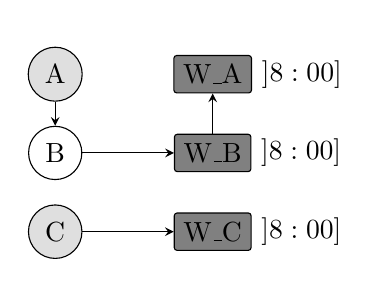
\begin{tikzpicture}
				\node[draw, circle, fill=gray!25, label=above:{$$}] (A)at(-1.5, 0.5) {A};
				\node[draw, circle, label=above:{$$}] (B)at(-1.5, -0.5) {B};
				\node[draw, circle, fill=gray!25, label=above:{$$}] (C)at(-1.5, -1.5) {C};
				\node[draw, rectangle, rounded corners=1pt, fill=gray!100, label=right:{$]8:00]$}] (WA)at(0.5, 0.5) {W\_A};
				\node[draw, rectangle, rounded corners=1pt, fill=gray!100, label=right:{$]8:00]$}] (WB)at(0.5, -0.5) {W\_B};
				\node[draw, rectangle, rounded corners=1pt, fill=gray!100, label=right:{$]8:00]$}] (WC)at(0.5, -1.5) {W\_C};
				\draw[->, >=stealth] (A) -- (B);
				\draw[->, >=stealth] (B) -- (WB);
				\draw[->, >=stealth] (WB) -- (WA);
				\draw[->, >=stealth] (C) -- (WC);
			\end{tikzpicture}
			\caption{Home-to-work trip}
		\end{subfigure}%
		\begin{subfigure}{.5\textwidth}
			\centering
			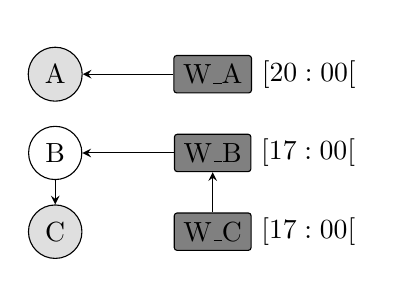
\begin{tikzpicture}
				\node[draw, circle, fill=gray!25, label=above:{$$}] (A)at(-1.5, 0.5) {A};
				\node[draw, circle, label=above:{$$}] (B)at(-1.5, -0.5) {B};
				\node[draw, circle, fill=gray!25, label=above:{$$}] (C)at(-1.5, -1.5) {C};
				\node[draw, rectangle, rounded corners=1pt, fill=gray!100, label=right:{$[20:00[$}] (WA)at(0.5, 0.5) {W\_A};
				\node[draw, rectangle, rounded corners=1pt, fill=gray!100, label=right:{$[17:00[$}] (WB)at(0.5, -0.5) {W\_B};
				\node[draw, rectangle, rounded corners=1pt, fill=gray!100, label=right:{$[17:00[$}] (WC)at(0.5, -1.5) {W\_C};
				\draw[->, >=stealth] (WA) -- (A);
				\draw[->, >=stealth] (WC) -- (WB);
				\draw[->, >=stealth] (WB) -- (B);
				\draw[->, >=stealth] (B) -- (C);
			\end{tikzpicture}
			\caption{Return trip}
		\end{subfigure}
		\footnotetext[1]{M Bruglieri - ‎2011}
	\end{figure}
	\end{frame}
	\subsection{One user several places}
	\begin{frame}
		\frametitle{Problem description: One user several places}
		\begin{figure}
		\centering
		\begin{subfigure}{.5\textwidth}
			\centering
			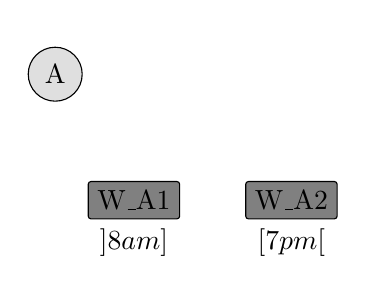
\begin{tikzpicture}
				\node[draw, circle, fill=gray!25, label=above:{$$}] (A)at(-1.5, 1) {A};
				\node[draw, rectangle, rounded corners=1pt, fill=gray!100, label=below:{$]8am]$}] (W1A)at(-0.5, -0.6) {W\_A1};
				\node[draw, rectangle, rounded corners=1pt, fill=gray!100, label=below:{$[7pm[$}] (W2A)at(1.5, -0.6) {W\_A2};
			\end{tikzpicture}
			\caption{ Data }
		\end{subfigure}%
		\begin{subfigure}{.5\textwidth}
			\centering
			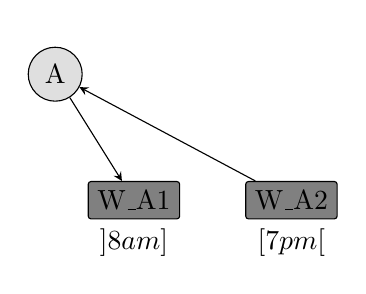
\begin{tikzpicture}
				\node[draw, circle, fill=gray!25, label=above:{$$}] (A)at(-1.5, 1) {A};
				\node[draw, rectangle, rounded corners=1pt, fill=gray!100, label=below:{$]8am]$}] (W1A)at(-0.5, -0.6) {W\_A1};
				\node[draw, rectangle, rounded corners=1pt, fill=gray!100, label=below:{$[7pm[$}] (W2A)at(1.5, -0.6) {W\_A2};
				\draw[->, >=stealth, above] (A) -- (W1A) node[midway] {$$};
				\draw[->, >=stealth, above] (W2A) -- (A) node[midway] {$$};
			\end{tikzpicture}
			\caption{ Solution }
		\end{subfigure}
		\end{figure}
		In the case the place of work is \textbf{not fixed}, or if the user planned an \textbf{external activity}.\newline
		The trip between the two workplaces is not managed by our system(company car, public transport, his car if he took it\dots ).\newline
		Same thing with homes, even if it is less frequent.
	\end{frame}
	\subsection{Latest arrival time}
	\begin{frame}
		\frametitle{Problem description: Latest arrival time}
		\begin{figure}
		\centering
		\begin{subfigure}{.5\textwidth}
			\centering
			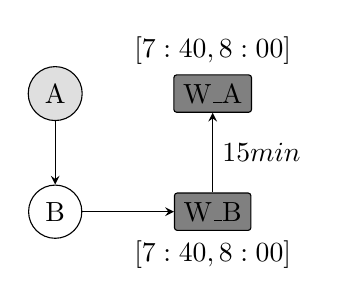
\begin{tikzpicture}
				\node[draw, circle, fill=gray!25, label=above:{$$}] (A)at(-1.5, 1) {A};
				\node[draw, circle, label=above:{$$}] (B)at(-1.5, -0.5) {B};
				\node[draw, rectangle, rounded corners=1pt, fill=gray!100, label=above:{$[7:40,8:00]$}] (WA)at(0.5, 1) {W\_A};
				\node[draw, rectangle, rounded corners=1pt, fill=gray!100, label=below:{$[7:40,8:00]$}] (WB)at(0.5, -0.5) {W\_B};
				\draw[->, >=stealth, above] (A) -- (B) node[midway] {$$};
				\draw[->, >=stealth, above] (B) -- (WB) node[midway] {$$};
				\draw[->, >=stealth, right] (WB) -- (WA) node[midway] {$15min$};
			\end{tikzpicture}
			\caption{Authorized advance = 20 min }
		\end{subfigure}%
		\begin{subfigure}{.5\textwidth}
			\centering
			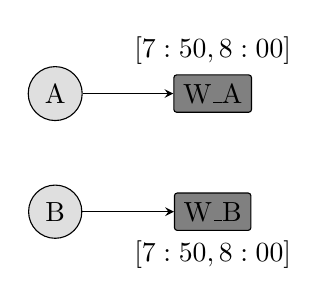
\begin{tikzpicture}
				\node[draw, circle, fill=gray!25, label=above:{$$}] (A)at(-1.5, 1) {A};
				\node[draw, circle, fill=gray!25, label=above:{$$}] (B)at(-1.5, -0.5) {B};
				\node[draw, rectangle, rounded corners=1pt, fill=gray!100, label=above:{$[7:50,8:00]$}] (WA)at(0.5, 1) {W\_A};
				\node[draw, rectangle, rounded corners=1pt, fill=gray!100, label=below:{$[7:50,8:00]$}] (WB)at(0.5, -0.5) {W\_B};
				\draw[->, >=stealth, above] (A) -- (WA) node[midway] {$$};
				\draw[->, >=stealth, above] (B) -- (WB) node[midway] {$$};
			\end{tikzpicture}
			\caption{Authorized advance = 10 min }
		\end{subfigure}
		\end{figure}
		The time window is of the form:\newline
		\textbf{[(Latest arrival time - Authorized advance),Latest arrival time]} \newline
		Similar thing after work, with the authorized wait.
	\end{frame}
	
	\subsection{Problem class}
	\begin{frame}
		\frametitle{Problem description: Problem class}
		\begin{figure}
		\centering
		\begin{subfigure}{.5\textwidth}
			\centering
			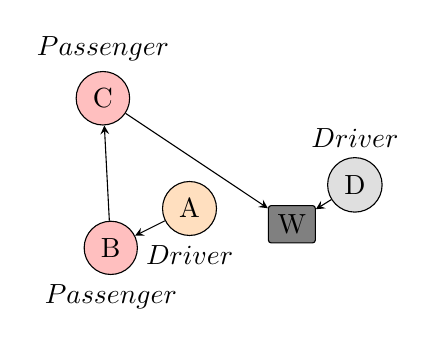
\begin{tikzpicture}
				\node[draw, circle, fill=orange!25, label=below:{$Driver$}] (A)at(-1.5, 0.2) {A};
				\node[draw, circle, fill=red!25, label=below:{$Passenger$}] (B)at(-2.5, -0.3) {B};
				\node[draw, circle, fill=red!25, label=above:{$Passenger$}] (C)at(-2.6, 1.6) {C};
				\node[draw, circle, fill=gray!25, label=above:{$Driver$}] (D)at(0.6, 0.5) {D};
				\node[draw, rectangle, rounded corners=1pt, fill=gray!100, label=above:{$$}] (W)at(-0.2, 0) {W};
				\draw[->, >=stealth] (A) -- (B);
				\draw[->, >=stealth] (B) -- (C);
				\draw[->, >=stealth] (C) -- (W);
				\draw[->, >=stealth] (D) -- (W);
			\end{tikzpicture}
			\caption{LCPP Day one}
		\end{subfigure}%
		\begin{subfigure}{.5\textwidth}
			\centering
			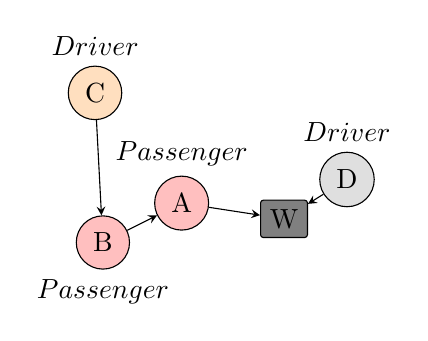
\begin{tikzpicture}
				\node[draw, circle, fill=red!25, label=above:{$Passenger$}] (A)at(-1.5, 0.2) {A};
				\node[draw, circle, fill=red!25, label=below:{$Passenger$}] (B)at(-2.5, -0.3) {B};
				\node[draw, circle, fill=orange!25, label=above:{$Driver$}] (C)at(-2.6, 1.6) {C};
				\node[draw, circle, fill=gray!25, label=above:{$Driver$}] (D)at(0.6, 0.5) {D};
				\node[draw, rectangle, rounded corners=1pt, fill=gray!100, label=above:{$$}] (W)at(-0.2, 0) {W};
				\draw[->, >=stealth] (C) -- (B);
				\draw[->, >=stealth] (B) -- (A);
				\draw[->, >=stealth] (A) -- (W);
				\draw[->, >=stealth] (D) -- (W);
			\end{tikzpicture}
			\caption{LCPP Day two}
		\end{subfigure}
		\end{figure}
		LCPP must have regular users with a long-term commitment. \newline
		We wanted a more flexible system, where users can change every day, and this class is called the DCPP.
		\footnotetext[1]{Vittorio Maniezzo, Roberto Wolfler Calvo - 2004}
	\end{frame}
	\subsection{State of the art}
	\begin{frame}
		\frametitle{Problem description: State of the art}
		\includegraphics[height=0.5\textwidth]{img/i_table.png}
		\footnotetext[1]{All references in the report Romain NAVARRO - 2018}
	\end{frame}
	
	%%%%%%%%%%%%%%%% MATHEMATICAL MODEL %%%%%%%%%%
	\section{Modeling}
	\subsection{Data}
	\begin{frame}
		\frametitle{Modeling: Data}
		\begin{figure}
		\centering
			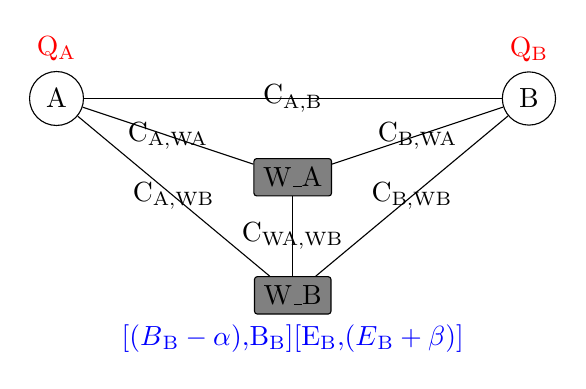
\begin{tikzpicture}
				\node[draw, circle, label={[red]{above}:Q\textsubscript{A}}] (A)at(-3, 1) {A};
				\node[draw, circle, label={[red]{above}:Q\textsubscript{B}}] (B)at(3, 1) {B};
				\node[draw, rectangle, rounded corners=1pt, fill=gray!100] (WA)at(0, 0) {W\_A};
				\node[draw, rectangle, rounded corners=1pt, fill=gray!100, label={[blue]{below}:[($B\textsubscript{B}-\alpha$),B\textsubscript{B}][E\textsubscript{B},($E\textsubscript{B}+\beta$)] }] (WB)at(0,-1.5) {W\_B};
				\draw (A) edge node{C\textsubscript{A,B}} (B);
				\draw (A) edge node{C\textsubscript{A,WB}} (WB);
				\draw (A) edge node{C\textsubscript{A,WA}} (WA);
				\draw (WA) edge node{C\textsubscript{WA,WB}} (WB);
				\draw (B) edge node{C\textsubscript{B,WB}} (WB);
				\draw (B) edge node{C\textsubscript{B,WA}} (WA);
			\end{tikzpicture}
		\end{figure}
	\end{frame}
	\begin{frame}
		\frametitle{Modeling: Data}
		Max travel time of a vertex v = direct travel time$\times (1+\gamma)+\delta$ 
		\begin{figure}
		\centering
		\begin{subfigure}{.5\textwidth}
			\centering
			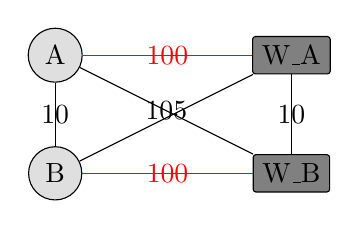
\begin{tikzpicture}
				\node[draw, fill=gray!25, circle] (A)at(-3, 1) {A};
				\node[draw, fill=gray!25, circle] (B)at(-3, -0.5) {B};
				\node[draw, rectangle, rounded corners=1pt, fill=gray!100] (WA)at(0, 1) {W\_A};
				\node[draw, rectangle, rounded corners=1pt, fill=gray!100] (WB)at(0,-0.5) {W\_B};
				\draw (A) edge node{10} (B);
				\draw (A) edge node{105} (WB);
				\draw (A) edge[red] node{100} (WA);
				\draw (WA) edge node{10} (WB);
				\draw (B) edge[red] node{100} (WB);
				\draw (B) edge node{} (WA);
			\end{tikzpicture}
			\caption{Authorized deviation = 0\% }
		\end{subfigure}%
		\begin{subfigure}{.5\textwidth}
			\centering
			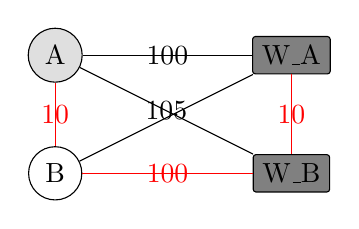
\begin{tikzpicture}
				\node[draw, fill=gray!25, circle] (A)at(-3, 1) {A};
				\node[draw, circle] (B)at(-3, -0.5) {B};
				\node[draw, rectangle, rounded corners=1pt, fill=gray!100] (WA)at(0, 1) {W\_A};
				\node[draw, rectangle, rounded corners=1pt, fill=gray!100] (WB)at(0,-0.5) {W\_B};
				\draw (A) edge[red] node{10} (B);
				\draw (A) edge node{105} (WB);
				\draw (A) edge node{100} (WA);
				\draw (WA) edge[red] node{10} (WB);
				\draw (B) edge[red] node{100} (WB);
				\draw (B) edge node{} (WA);
			\end{tikzpicture}
			\caption{Authorized deviation = 20\% }
		\end{subfigure}
		\end{figure}
	\end{frame}
	
	\subsection{Decision variables}
	\begin{frame}
		\frametitle{Modeling: Decision variables}
		\begin{figure}
			\centering
			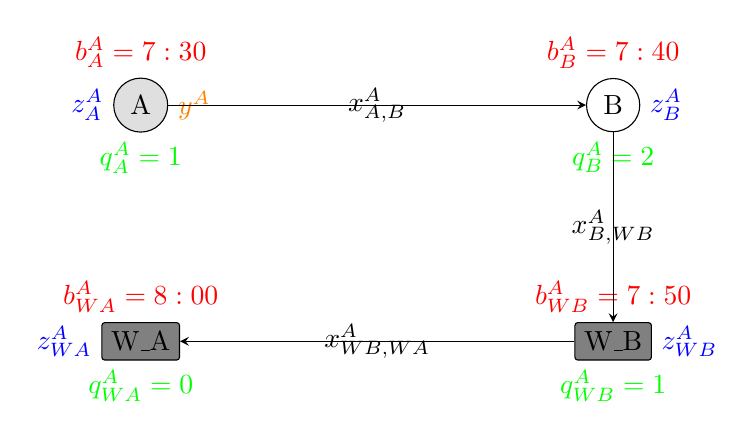
\begin{tikzpicture}
				\node[draw, circle, fill=gray!25, label={[red]{above}:$b^{A}_{A}=7:30$}, label={[blue]{left}:$z^{A}_{A}$}, label={[green]{below}:$q^{A}_{A}=1$}, label={[orange]{right}:$y^{A}$}] (A)at(-3, 1) {A};
				\node[draw, circle, label={[red]{above}:$b^{A}_{B}=7:40$}, label={[blue]{right}:$z^{A}_{B}$}, label={[green]{below}:$q^{A}_{B}=2$}] (B)at(3, 1) {B};
				\node[draw, rectangle, rounded corners=1pt, fill=gray!100, label={[red]{above}:$b^{A}_{WA}=8:00$}, label={[blue]{left}:$z^{A}_{WA}$}, label={[green]{below}:$q^{A}_{WA}=0$}] (WA)at(-3, -2) {W\_A};
				\node[draw, rectangle, rounded corners=1pt, fill=gray!100, label={[red]{above}:$b^{A}_{WB}=7:50$}, label={[blue]{right}:$z^{A}_{WB}$}, label={[green]{below}:$q^{A}_{WB}=1$}] (WB)at(3, -2) {W\_B};
				\draw[->, >=stealth] (A) -- (B) node[midway] {$x^{A}_{A,B}$};
				\draw[->, >=stealth] (B) -- (WB) node[midway] {$x^{A}_{B,WB}$};
				\draw[->, >=stealth] (WB) -- (WA) node[midway] {$x^{A}_{WB,WA}$};
			\end{tikzpicture}
		\end{figure}
	\end{frame}
	\subsection{Constraints summary}
	\begin{frame}
		\frametitle{Modeling: Constraints summary}
		\textbf{Path constraints:} (section 4.4.1 p32-33)
		\begin{itemize}
			\item Only a driver can pick-up passengers, and pick himself up
			\item A passenger picked up by a driver must be dropped by that driver
			\item An user never leaves his destination
		\end{itemize}
		\textbf{Time constraints:} (section 4.4.1 p33-34)
		\begin{itemize}
			\item The passage time at each vertex is precisely sequenced, respecting the time windows and max travel time constraints
		\end{itemize}
		\textbf{Capacity constraints:} (section 4.4.1 p34)
		\begin{itemize}
			\item The car's capacity at each vertex is precisely sequenced, and never exceeds its maximum capacity
		\end{itemize}
		\footnotetext[1]{Hossein Karimi - 2018}
	\end{frame}
	\subsection{Resolution process}
	\begin{frame}
		\frametitle{Modeling: Resolution process}
		\begin{figure}
		\centering
			\includegraphics[width=.8\textwidth]{img/i_presflowchart}
		\end{figure}
	\end{frame}
	%%%%%%%%%%%% EXPERIMENTS %%%%%%%%%%%%
	\section{Experiments}
	\subsection{Protocol}
	\begin{frame}
		\frametitle{Experiments : Protocol}
		The PC used for the experiments:
		\begin{itemize}
		\item Operating System: \textbf{Windows 10 Professional 64-bit version}. 
		\item Code language: \textbf{JAVA }
		\item Solver: \textbf{CPLEX}
		\item RAM quantity: \textbf{8GB}
		\item CPU: \textbf{Intel Core i5-4690 CPU 3.50 GHz}
		\end{itemize}
		All available at the following web address: \url{https://github.com/NeoKa4ra/CarPoolingInternship}
	\end{frame}
	\subsection{General parameters}
	\begin{frame}
		\frametitle{Experiments: General parameters}
		\begin{itemize}
			\item \textbf{Generator mode}: \textcolor{red}{Associated} Associated or dissociated program
			\item \textbf{Instances mode}: \textcolor{red}{Change} Does the instance have to change between each execution?
			\item \textbf{Number of runs} \textcolor{red}{30}
			\item \textbf{Maximum execution time} \textcolor{red}{6 minutes}
			\item \textbf{Maximum number of executions} \textcolor{red}{30}
		\end{itemize}
	\end{frame}
	\subsection{Linear program parameters}
	\begin{frame}
		\frametitle{Experiments: Linear program parameters}
		\begin{itemize}
			\item \textbf{Maximum advance time} \textcolor{red}{30 minutes}
			\item \textbf{Maximum waiting time} \textcolor{red}{15 minutes}
			\item \textbf{Percentage deviation} \textcolor{red}{20\%}
			\item \textbf{Fixed deviation value} \textcolor{red}{5}
		\end{itemize}
	\end{frame}
	\subsection{Instances parameters}
	\begin{frame}
		\frametitle{Experiments: Instances parameters}
		\begin{itemize}
			\item \textbf{Instance mode}: \textcolor{red}{3 random cities and random workplaces} Predefined cities, all random\dots
			\item \textbf{Number of users} \textcolor{red}{20}
			\item \textbf{List of predefined cities and workplaces} \textcolor{red}{None}
			\item \textbf{Probability of having a second workplace} \textcolor{red}{20\%}
			\item \textbf{Probability of having a second home} \textcolor{red}{5\%}
			\item \textbf{Ranges in which the schedules will be generated } \textcolor{red}{[8am,9am] and [4pm,9pm]}
		\end{itemize}
	\end{frame}
	\subsection{Overall results}
	\begin{frame}
		\frametitle{Experiments: Overall results}
		\begin{figure}
			\centering
			\includegraphics[width=\textwidth]{img/compiledResults/12}
			\caption{Vary users}
		\end{figure}
	\end{frame}
	\begin{frame}
		\frametitle{Experiments: Overall results}
		\begin{figure}
			\centering
			\includegraphics[width=\textwidth]{img/compiledResults/7}
			\caption{Vary the deviation percentage with 19 users}
		\end{figure}
	\end{frame}
	\subsection{Fill rate}
	\begin{frame}
		\frametitle{Experiments: Fill rate}
		Vehicle fill rate: Average number of people per car \newline
		Home-to-work daily commuting in France: from \textbf{1.1 to 1.2} people per car.
		\begin{center}
		\begin{tabular}{|l|c|c|r|}
			\hline
			Hours generation range & 5:00 & 1:00 & 0:00 \\
			\hline
			Mean & 1.14 & 1.38 & 1.81 \\
			Median & 1.15 & 1.35 & 1.86 \\
			Standard deviation & 0.09 & 0.12 & 0.21 \\
			\hline
		\end{tabular}
		\end{center}
		The more users we have with close working hours, the higher the fill rate is .
		\footnotetext[1]{Quel est le taux d’occupation d'une voiture ? - www.futura-sciences.com}
	\end{frame}
	\subsection{Same user pool}
	\begin{frame}
		\frametitle{Experiments : Same user pool}
		Same pool: much lower execution time 
		\begin{center}
		\captionof{table}{Objective value with 5 users}
		\begin{tabular}{|l|c|r|}
			\hline
			Name of the data & LP & LPSP \\
			\hline
			Mean & 48.96 & 50.04 \\
			Median & 48.5 & 50.5 \\
			Standard deviation & 15.26 & 15.32 \\
			\hline
		\end{tabular}
		\end{center}
		\begin{center}
		\captionof{table}{Objective value with 10 users}
		\begin{tabular}{|l|c|r|}
			\hline
			Name of the data & LP & LPSP \\
			\hline
			Mean & 92.00 & 98.90 \\
			Median & 88.00 & 95.5 \\
			Standard deviation & 19.32 & 20.58 \\
			\hline
		\end{tabular}
		\end{center}
		Objective difference with: 5 users: 2.20\% ,10 users: 7.5\%
	\end{frame}
	\subsection{Limits of the model}
	\begin{frame}
		\frametitle{Experiments: Limits of the model}
		We decided that having a maximum GAP of 2\% on average was appropriate. \newline
		Less than 2\% of GAP on 1 hour for 25 users.\newline
		Less than 10\% of GAP on 1 hour for 30 users. \newline
		We can manage up to 25 people with the default configuration.
	\end{frame}
	\subsection{The case of Grenoble}
	\begin{frame}
		\frametitle{Experiments: The case of Grenoble}
		\begin{figure}
		\centering
			\includegraphics[height=0.5\textwidth]{img/i_grenoble.png}
		\caption{Mountains around Grenoble city}
		\label{fig:Mountains around Grenoble city}
	\end{figure}
	\end{frame}
	\begin{frame}
		\frametitle{Experiments: The case of Grenoble}
		\begin{figure}
		\centering
		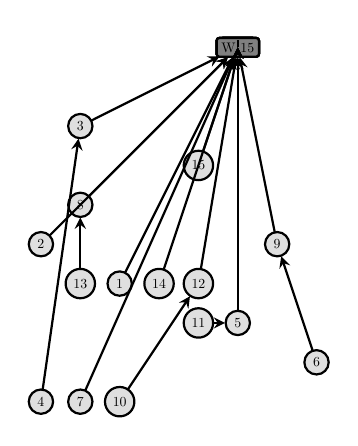
\begin{tikzpicture}[thick,scale=0.5, every node/.style={transform shape}]
			\node[draw,circle,fill=gray!25,label=above:{$$}] (1)at(-3.0,-6.0) {1};
			\node[draw,circle,fill=gray!25,label=above:{$$}] (2)at(-5.0,-5.0) {2};
			\node[draw,circle,fill=gray!25,label=above:{$$}] (3)at(-4.0,-2.0) {3};
			\node[draw,circle,fill=gray!25,label=above:{$$}] (4)at(-5.0,-9.0) {4};
			\node[draw,circle,fill=gray!25,label=above:{$$}] (5)at(0.0,-7.0) {5};
			\node[draw,circle,fill=gray!25,label=above:{$$}] (6)at(2.0,-8.0) {6};
			\node[draw,circle,fill=gray!25,label=above:{$$}] (7)at(-4.0,-9.0) {7};
			\node[draw,circle,fill=gray!25,label=above:{$$}] (8)at(-4.0,-4.0) {8};
			\node[draw,circle,fill=gray!25,label=above:{$$}] (9)at(1.0,-5.0) {9};
			\node[draw,circle,fill=gray!25,label=above:{$$}] (10)at(-3.0,-9.0) {10};
			\node[draw,circle,fill=gray!25,label=above:{$$}] (11)at(-1.0,-7.0) {11};
			\node[draw,circle,fill=gray!25,label=above:{$$}] (12)at(-1.0,-6.0) {12};
			\node[draw,circle,fill=gray!25,label=above:{$$}] (13)at(-4.0,-6.0) {13};
			\node[draw,circle,fill=gray!25,label=above:{$$}] (14)at(-2.0,-6.0) {14};
			\node[draw,circle,fill=gray!25,label=above:{$$}] (15)at(-1.0,-3.0) {15};
			\node[draw,rectangle,rounded corners=1pt,fill=gray!100,label=above:{$$}] (W1)at(0.0,0.0) {W\_1};
			\node[draw,rectangle,rounded corners=1pt,fill=gray!100,label=above:{$$}] (W2)at(0.0,0.0) {W\_2};
			\node[draw,rectangle,rounded corners=1pt,fill=gray!100,label=above:{$$}] (W3)at(0.0,0.0) {W\_3};
			\node[draw,rectangle,rounded corners=1pt,fill=gray!100,label=above:{$$}] (W4)at(0.0,0.0) {W\_4};
			\node[draw,rectangle,rounded corners=1pt,fill=gray!100,label=above:{$$}] (W5)at(0.0,0.0) {W\_5};
			\node[draw,rectangle,rounded corners=1pt,fill=gray!100,label=above:{$$}] (W6)at(0.0,0.0) {W\_6};
			\node[draw,rectangle,rounded corners=1pt,fill=gray!100,label=above:{$$}] (W7)at(0.0,0.0) {W\_7};
			\node[draw,rectangle,rounded corners=1pt,fill=gray!100,label=above:{$$}] (W8)at(0.0,0.0) {W\_8};
			\node[draw,rectangle,rounded corners=1pt,fill=gray!100,label=above:{$$}] (W9)at(0.0,0.0) {W\_9};
			\node[draw,rectangle,rounded corners=1pt,fill=gray!100,label=above:{$$}] (W10)at(0.0,0.0) {W\_10};
			\node[draw,rectangle,rounded corners=1pt,fill=gray!100,label=above:{$$}] (W11)at(0.0,0.0) {W\_11};
			\node[draw,rectangle,rounded corners=1pt,fill=gray!100,label=above:{$$}] (W12)at(0.0,0.0) {W\_12};
			\node[draw,rectangle,rounded corners=1pt,fill=gray!100,label=above:{$$}] (W13)at(0.0,0.0) {W\_13};
			\node[draw,rectangle,rounded corners=1pt,fill=gray!100,label=above:{$$}] (W14)at(0.0,0.0) {W\_14};
			\node[draw,rectangle,rounded corners=1pt,fill=gray!100,label=above:{$$}] (W15)at(0.0,0.0) {W\_15};
			\draw[->,>=stealth] (1) -- (W1);
			\draw[->,>=stealth] (2) -- (W2);
			\draw[->,>=stealth] (3) -- (W3);
			\draw[->,>=stealth] (4) -- (3);
			\draw[->,>=stealth] (W3) -- (W4);
			\draw[->,>=stealth] (6) -- (9);
			\draw[->,>=stealth] (9) -- (W9);
			\draw[->,>=stealth] (W9) -- (W6);
			\draw[->,>=stealth] (7) -- (W7);
			\draw[->,>=stealth] (10) -- (12);
			\draw[->,>=stealth] (12) -- (W12);
			\draw[->,>=stealth] (W12) -- (W10);
			\draw[->,>=stealth] (5) -- (W5);
			\draw[->,>=stealth] (11) -- (5);
			\draw[->,>=stealth] (W5) -- (W11);
			\draw[->,>=stealth] (8) -- (W8);
			\draw[->,>=stealth] (13) -- (8);
			\draw[->,>=stealth] (W8) -- (W13);
			\draw[->,>=stealth] (14) -- (W14);
			\draw[->,>=stealth] (15) -- (W15);
		\end{tikzpicture}
		\caption{Home-to-work: VIZILLE PONT-DE-CLAIX VIF}
	\end{figure}
	\end{frame}
	
	\begin{frame}
		\frametitle{Experiments: The case of Grenoble}
		\begin{figure}
		\centering
		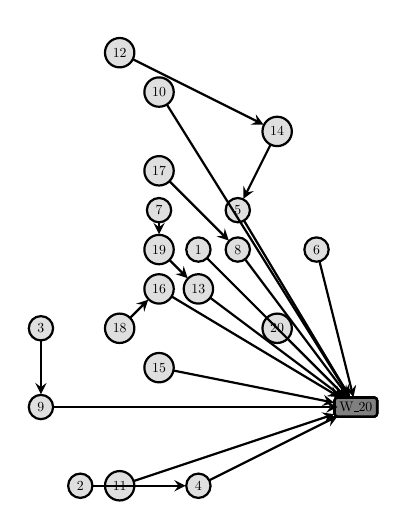
\begin{tikzpicture}[thick,scale=0.5, every node/.style={transform shape}]
			\node[draw,circle,fill=gray!25,label=above:{$$}] (1)at(-4.0,4.0) {1};
			\node[draw,circle,fill=gray!25,label=above:{$$}] (2)at(-7.0,-2.0) {2};
			\node[draw,circle,fill=gray!25,label=above:{$$}] (3)at(-8.0,2.0) {3};
			\node[draw,circle,fill=gray!25,label=above:{$$}] (4)at(-4.0,-2.0) {4};
			\node[draw,circle,fill=gray!25,label=above:{$$}] (5)at(-3.0,5.0) {5};
			\node[draw,circle,fill=gray!25,label=above:{$$}] (6)at(-1.0,4.0) {6};
			\node[draw,circle,fill=gray!25,label=above:{$$}] (7)at(-5.0,5.0) {7};
			\node[draw,circle,fill=gray!25,label=above:{$$}] (8)at(-3.0,4.0) {8};
			\node[draw,circle,fill=gray!25,label=above:{$$}] (9)at(-8.0,0.0) {9};
			\node[draw,circle,fill=gray!25,label=above:{$$}] (10)at(-5.0,8.0) {10};
			\node[draw,circle,fill=gray!25,label=above:{$$}] (11)at(-6.0,-2.0) {11};
			\node[draw,circle,fill=gray!25,label=above:{$$}] (12)at(-6.0,9.0) {12};
			\node[draw,circle,fill=gray!25,label=above:{$$}] (13)at(-4.0,3.0) {13};
			\node[draw,circle,fill=gray!25,label=above:{$$}] (14)at(-2.0,7.0) {14};
			\node[draw,circle,fill=gray!25,label=above:{$$}] (15)at(-5.0,1.0) {15};
			\node[draw,circle,fill=gray!25,label=above:{$$}] (16)at(-5.0,3.0) {16};
			\node[draw,circle,fill=gray!25,label=above:{$$}] (17)at(-5.0,6.0) {17};
			\node[draw,circle,fill=gray!25,label=above:{$$}] (18)at(-6.0,2.0) {18};
			\node[draw,circle,fill=gray!25,label=above:{$$}] (19)at(-5.0,4.0) {19};
			\node[draw,circle,fill=gray!25,label=above:{$$}] (20)at(-2.0,2.0) {20};
			\node[draw,rectangle,rounded corners=1pt,fill=gray!100,label=above:{$$}] (W1)at(0.0,0.0) {W\_1};
			\node[draw,rectangle,rounded corners=1pt,fill=gray!100,label=above:{$$}] (W2)at(0.0,0.0) {W\_2};
			\node[draw,rectangle,rounded corners=1pt,fill=gray!100,label=above:{$$}] (W3)at(0.0,0.0) {W\_3};
			\node[draw,rectangle,rounded corners=1pt,fill=gray!100,label=above:{$$}] (W4)at(0.0,0.0) {W\_4};
			\node[draw,rectangle,rounded corners=1pt,fill=gray!100,label=above:{$$}] (W5)at(0.0,0.0) {W\_5};
			\node[draw,rectangle,rounded corners=1pt,fill=gray!100,label=above:{$$}] (W6)at(0.0,0.0) {W\_6};
			\node[draw,rectangle,rounded corners=1pt,fill=gray!100,label=above:{$$}] (W7)at(0.0,0.0) {W\_7};
			\node[draw,rectangle,rounded corners=1pt,fill=gray!100,label=above:{$$}] (W8)at(0.0,0.0) {W\_8};
			\node[draw,rectangle,rounded corners=1pt,fill=gray!100,label=above:{$$}] (W9)at(0.0,0.0) {W\_9};
			\node[draw,rectangle,rounded corners=1pt,fill=gray!100,label=above:{$$}] (W10)at(0.0,0.0) {W\_10};
			\node[draw,rectangle,rounded corners=1pt,fill=gray!100,label=above:{$$}] (W11)at(0.0,0.0) {W\_11};
			\node[draw,rectangle,rounded corners=1pt,fill=gray!100,label=above:{$$}] (W12)at(0.0,0.0) {W\_12};
			\node[draw,rectangle,rounded corners=1pt,fill=gray!100,label=above:{$$}] (W13)at(0.0,0.0) {W\_13};
			\node[draw,rectangle,rounded corners=1pt,fill=gray!100,label=above:{$$}] (W14)at(0.0,0.0) {W\_14};
			\node[draw,rectangle,rounded corners=1pt,fill=gray!100,label=above:{$$}] (W15)at(0.0,0.0) {W\_15};
			\node[draw,rectangle,rounded corners=1pt,fill=gray!100,label=above:{$$}] (W16)at(0.0,0.0) {W\_16};
			\node[draw,rectangle,rounded corners=1pt,fill=gray!100,label=above:{$$}] (W17)at(0.0,0.0) {W\_17};
			\node[draw,rectangle,rounded corners=1pt,fill=gray!100,label=above:{$$}] (W18)at(0.0,0.0) {W\_18};
			\node[draw,rectangle,rounded corners=1pt,fill=gray!100,label=above:{$$}] (W19)at(0.0,0.0) {W\_19};
			\node[draw,rectangle,rounded corners=1pt,fill=gray!100,label=above:{$$}] (W20)at(0.0,0.0) {W\_20};
			\draw[->,>=stealth] (1) -- (W1);
			\draw[->,>=stealth] (2) -- (4);
			\draw[->,>=stealth] (4) -- (W4);
			\draw[->,>=stealth] (3) -- (9);
			\draw[->,>=stealth] (9) -- (W9);
			\draw[->,>=stealth] (6) -- (W6);
			\draw[->,>=stealth] (7) -- (19);
			\draw[->,>=stealth] (13) -- (W13);
			\draw[->,>=stealth] (19) -- (13);
			\draw[->,>=stealth] (10) -- (W10);
			\draw[->,>=stealth] (11) -- (W11);
			\draw[->,>=stealth] (5) -- (W5);
			\draw[->,>=stealth] (12) -- (14);
			\draw[->,>=stealth] (14) -- (5);
			\draw[->,>=stealth] (15) -- (W15);
			\draw[->,>=stealth] (8) -- (W8);
			\draw[->,>=stealth] (17) -- (8);
			\draw[->,>=stealth] (16) -- (W16);
			\draw[->,>=stealth] (18) -- (16);
			\draw[->,>=stealth] (20) -- (W20);
			\end{tikzpicture}
		\caption{Home-to-work: VOIRON VINAY SAINT-LAURENT-DU-PONT}
	\end{figure}
	\end{frame}
	
	\begin{frame}
		\frametitle{Experiments: The case of Grenoble}
		\begin{figure}
		\centering
		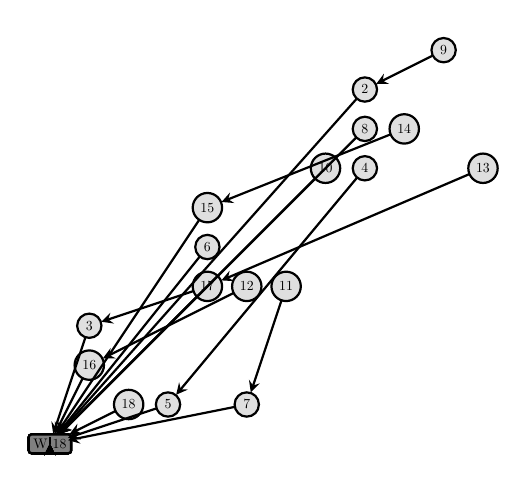
\begin{tikzpicture}[thick,scale=0.5, every node/.style={transform shape}]
			\node[draw,circle,fill=gray!25,label=above:{$$}] (1)at(4.0,4.0) {1};
			\node[draw,circle,fill=gray!25,label=above:{$$}] (2)at(8.0,9.0) {2};
			\node[draw,circle,fill=gray!25,label=above:{$$}] (3)at(1.0,3.0) {3};
			\node[draw,circle,fill=gray!25,label=above:{$$}] (4)at(8.0,7.0) {4};
			\node[draw,circle,fill=gray!25,label=above:{$$}] (5)at(3.0,1.0) {5};
			\node[draw,circle,fill=gray!25,label=above:{$$}] (6)at(4.0,5.0) {6};
			\node[draw,circle,fill=gray!25,label=above:{$$}] (7)at(5.0,1.0) {7};
			\node[draw,circle,fill=gray!25,label=above:{$$}] (8)at(8.0,8.0) {8};
			\node[draw,circle,fill=gray!25,label=above:{$$}] (9)at(10.0,10.0) {9};
			\node[draw,circle,fill=gray!25,label=above:{$$}] (10)at(7.0,7.0) {10};
			\node[draw,circle,fill=gray!25,label=above:{$$}] (11)at(6.0,4.0) {11};
			\node[draw,circle,fill=gray!25,label=above:{$$}] (12)at(5.0,4.0) {12};
			\node[draw,circle,fill=gray!25,label=above:{$$}] (13)at(11.0,7.0) {13};
			\node[draw,circle,fill=gray!25,label=above:{$$}] (14)at(9.0,8.0) {14};
			\node[draw,circle,fill=gray!25,label=above:{$$}] (15)at(4.0,6.0) {15};
			\node[draw,circle,fill=gray!25,label=above:{$$}] (16)at(1.0,2.0) {16};
			\node[draw,circle,fill=gray!25,label=above:{$$}] (17)at(4.0,4.0) {17};
			\node[draw,circle,fill=gray!25,label=above:{$$}] (18)at(2.0,1.0) {18};
			\node[draw,rectangle,rounded corners=1pt,fill=gray!100,label=above:{$$}] (W1)at(0.0,0.0) {W\_1};
			\node[draw,rectangle,rounded corners=1pt,fill=gray!100,label=above:{$$}] (W2)at(0.0,0.0) {W\_2};
			\node[draw,rectangle,rounded corners=1pt,fill=gray!100,label=above:{$$}] (W3)at(0.0,0.0) {W\_3};
			\node[draw,rectangle,rounded corners=1pt,fill=gray!100,label=above:{$$}] (W4)at(0.0,0.0) {W\_4};
			\node[draw,rectangle,rounded corners=1pt,fill=gray!100,label=above:{$$}] (W5)at(0.0,0.0) {W\_5};
			\node[draw,rectangle,rounded corners=1pt,fill=gray!100,label=above:{$$}] (W6)at(0.0,0.0) {W\_6};
			\node[draw,rectangle,rounded corners=1pt,fill=gray!100,label=above:{$$}] (W7)at(0.0,0.0) {W\_7};
			\node[draw,rectangle,rounded corners=1pt,fill=gray!100,label=above:{$$}] (W8)at(0.0,0.0) {W\_8};
			\node[draw,rectangle,rounded corners=1pt,fill=gray!100,label=above:{$$}] (W9)at(0.0,0.0) {W\_9};
			\node[draw,rectangle,rounded corners=1pt,fill=gray!100,label=above:{$$}] (W10)at(0.0,0.0) {W\_10};
			\node[draw,rectangle,rounded corners=1pt,fill=gray!100,label=above:{$$}] (W11)at(0.0,0.0) {W\_11};
			\node[draw,rectangle,rounded corners=1pt,fill=gray!100,label=above:{$$}] (W12)at(0.0,0.0) {W\_12};
			\node[draw,rectangle,rounded corners=1pt,fill=gray!100,label=above:{$$}] (W13)at(0.0,0.0) {W\_13};
			\node[draw,rectangle,rounded corners=1pt,fill=gray!100,label=above:{$$}] (W14)at(0.0,0.0) {W\_14};
			\node[draw,rectangle,rounded corners=1pt,fill=gray!100,label=above:{$$}] (W15)at(0.0,0.0) {W\_15};
			\node[draw,rectangle,rounded corners=1pt,fill=gray!100,label=above:{$$}] (W16)at(0.0,0.0) {W\_16};
			\node[draw,rectangle,rounded corners=1pt,fill=gray!100,label=above:{$$}] (W17)at(0.0,0.0) {W\_17};
			\node[draw,rectangle,rounded corners=1pt,fill=gray!100,label=above:{$$}] (W18)at(0.0,0.0) {W\_18};
			\draw[->,>=stealth] (1) -- (W1);
			\draw[->,>=stealth] (4) -- (5);
			\draw[->,>=stealth] (5) -- (W5);
			\draw[->,>=stealth] (W5) -- (W4);
			\draw[->,>=stealth] (6) -- (W6);
			\draw[->,>=stealth] (8) -- (W8);
			\draw[->,>=stealth] (2) -- (W2);
			\draw[->,>=stealth] (9) -- (2);
			\draw[->,>=stealth] (W2) -- (W9);
			\draw[->,>=stealth] (10) -- (W10);
			\draw[->,>=stealth] (7) -- (W7);
			\draw[->,>=stealth] (11) -- (7);
			\draw[->,>=stealth] (W7) -- (W11);
			\draw[->,>=stealth] (12) -- (16);
			\draw[->,>=stealth] (16) -- (W16);
			\draw[->,>=stealth] (W16) -- (W12);
			\draw[->,>=stealth] (3) -- (W3);
			\draw[->,>=stealth] (13) -- (17);
			\draw[->,>=stealth] (17) -- (3);
			\draw[->,>=stealth] (W3) -- (W17);
			\draw[->,>=stealth] (W17) -- (W13);
			\draw[->,>=stealth] (14) -- (15);
			\draw[->,>=stealth] (15) -- (W15);
			\draw[->,>=stealth] (W15) -- (W14);
			\draw[->,>=stealth] (18) -- (W18);
			\end{tikzpicture}
		\caption{Home-to-work: PONTCHARRA LE-TOUVET CROLLES}
		\label{fig:Return trip for the cities : PONTCHARRA LE-TOUVET CROLLES}
	\end{figure}
	\end{frame}
	%%%%%%%%%%%%%%%% CONCLUSION %%%%%%%%%%%%
	\section*{Conclusion}
	\begin{frame}
		\frametitle{Conclusion}
		Is not more complex than common CPP:
		\begin{itemize}
			\item Return Management
			\item One user with multiple workplaces
			\item Have respected and respectable schedules
		\end{itemize}
		Set up prospects:
		\begin{itemize}
			\item Parking relay before entering the valleys
		\end{itemize}
		Resolution prospects:
		\begin{itemize}
			\item Manage more users with a heuristic
			\begin{itemize}
				\item Find the heuristics most appropriate to the particularities of Grenoble
			\end{itemize}
		\end{itemize}
	\end{frame}
\end{document}